\documentclass[../main.tex]{subfiles}

\begin{document}

\section{Force model}\label{sec:force}
So far we have only considered the gravitational force acting between point masses. In reality, the Earth is not a point mass, neither a spherically symmetric mass distribution. In this section we will delve into the details of a more realistic model of the Earth's gravitational field.
\subsection{Geopotential model}
\subsubsection{Continuous distribution of mass}
In \cref{sec:twoBody} we have seen that the motion of a body orbiting another one can be described by a conic section. However, we have not been concerned about the mass distribution of the large body, in our case the Earth. In this section we will see that the motion of the smaller body, the satellite, is slightly perturbed by the mass distribution of the Earth as well as the presence of other forces such as atmospheric drag, solar radiation pressure, and the gravitational pull of the Moon and Sun, which we will talk later on. Even though, the perturbations are relatively small and the orbits of the satellites are still approximating ellipses.

Consider a body confined in a compact region $\Omega\subseteq\RR$ with a continuous density of mass $\rho:\Omega\to\RR$. We would like to know the gravitational pull on a point mass $m$ located at position $\vf{r}$ from the center of mass of the body. To do this we can discretize the body $\Omega$ in a set of cubes $m_{i,j,k}$ each of volume $\frac{1}{n_xn_yn_z}$ and density $\rho(\frac{i}{n_x},\frac{j}{n_y},\frac{k}{n_z})=:\rho_{i,j,k}$, where $n_x$, $n_y$, and $n_z$ are the number of cubes in the $x$, $y$, and $z$ directions, respectively. The total gravitational acceleration $\vf{g}$ exerted on $m$ is the sum of the contributions of all the forces exerted by the cubes (considered as point masses) and it is given by:
\begin{equation}\label{eq:riemann_sum}
  \vf{g}=-\sum_{i=0}^{n_x}\sum_{j=0}^{n_y}\sum_{k=0}^{n_z}\frac{m_{i,j,k}}{\norm{\vf{r}-\vf{s}_{i,j,k}}^3}(\vf{r}-\vf{s}_{i,j,k})=-\sum_{i=0}^{n_x}\sum_{j=0}^{n_y}\sum_{k=0}^{n_z}\frac{\rho_{i,j,k}}{\norm{\vf{r}-\vf{s}_{i,j,k}}^3}(\vf{r}-\vf{s}_{i,j,k})\frac{1}{n_xn_yn_z}
\end{equation}
where $\vf{s}_{i,j,k}=(\frac{i}{n_x},\frac{j}{n_y},\frac{k}{n_z})$ (in Cartesian coordinates). Note that \cref{eq:riemann_sum} is a Riemann sum and so letting $n_x,n_y,n_z\to\infty$ we get:
\begin{equation}\label{eq:limit}
  \vf{g}=-\int_{\Omega}\frac{\rho(\vf{s})}{\norm{\vf{r}-\vf{s}}^3}(\vf{r}-\vf{s})\dd^3{\vf{s}}
\end{equation}
where $\dd^3{\vf{s}}:=\dd{x'}\dd{y'}\dd{z'}$, if $\vf{s}=(x',y',z')$.
\begin{theorem}\label{thm:conservative}
  Let $\Omega$ be a compact region in $\RR^3$ with a continuous density of mass $\rho:\Omega\to\RR$. Then, the gravitational acceleration field $\vf{g}$ is conservative. That is, there exists a function $f:\RR^3\rightarrow\RR$ such that $\vf{g}=\grad f$.
\end{theorem}
\begin{proof}
  An easy computation shows that fixed $\vf{s}\in\RR^3$ we have:
  \begin{equation}
    \grad\left(\frac{1}{\norm{\vf{r}-\vf{s}}}\right)=-\frac{1}{\norm{\vf{r}-\vf{s}}^3}(\vf{r}-\vf{s})
  \end{equation}
  So we need to justify if the following exchange between the gradient and the integral is correct:
  \begin{equation}
    \vf{g}=-\int_{\Omega}\frac{\rho(\vf{s})}{\norm{\vf{r}-\vf{s}}^3}(\vf{r}-\vf{s})\dd^3{\vf{s}}=\int_{\Omega}\rho(\vf{s})\grad\left(\frac{1}{\norm{\vf{r}-\vf{s}}}\right)\dd^3{\vf{s}}=\grad\int_{\Omega}\frac{\rho(\vf{s})}{\norm{\vf{r}-\vf{s}}}\dd^3{\vf{s}}
  \end{equation}
  Without loss of generality it suffices to justify that
  \begin{equation}\label{eq:exchangeDivInt}
    \pdv{}{x}\int_{\Omega}\frac{\rho(\vf{s})}{\norm{\vf{r}-\vf{s}}}\dd^3{\vf{s}}=\int_{\Omega}\pdv{}{x}\left(\frac{\rho(\vf{s})}{\norm{\vf{r}-\vf{s}}}\right)\dd^3{\vf{s}}
  \end{equation}
  assuming $\vf{r}=(x,y,z)$ and $\vf{s}=(x',y',z')$. In order to apply the theorem of derivation under the integral sign we need to control $\pdv{}{x}\left(\frac{\rho(\vf{s})}{\norm{\vf{r}-\vf{s}}}\right)=-\rho(\vf{s})\frac{x-x'}{\norm{\vf{r}-\vf{s}}^3}$ by an integrable function $h(\vf{s})$. Using spherical coordinates centered at $\vf{r}$ and writing ${(\vf{r}-\vf{s})}_{\mathrm{sph}}=(\rho_{\vf{r}},\theta,\phi)$, the integrand to bound becomes (in spherical coordinates):
  \begin{equation}
    \abs{-\rho(\vf{s})\frac{x-x'}{\norm{\vf{r}-\vf{s}}^3}{\rho_{\vf{r}}}^2\sin\phi}=\abs{\rho(\vf{s})}\abs{\frac{{\rho_{\vf{r}}}\cos\theta\sin\phi}{{\rho_{\vf{r}}}^3}{\rho_{\vf{r}}}^2\sin\phi}\leq \abs{\rho(\vf{s})}\leq K
  \end{equation}
  where the last inequality follows for certain $K\in\RR$ by Weierstra\ss\ theorem ($\rho$ is continuous and $\Omega$ is compact). Thus, since $h(\vf{s})=K$ is integrable, because $\Omega$ is bounded, the equality of \cref{eq:exchangeDivInt} is licit.
\end{proof}
Physically speaking, the gravitational force $\vf{F}$ being conservative means that the work $W$ done by the force along a path $C$
\begin{equation}
  W=\int_C\vf{F}\cdot\dd{\vf{s}}
\end{equation}
depends only on the initial and final positions of it. Moreover, due to historical reasons, we will write $\vf{g}=-\grad V$ (with the minus sign) and call $V$ the \emph{gravitational potential}. The minus sign is chosen according the convention that work done by gravitational forces decreases the potential.
\subsubsection{Laplace's equation for \texorpdfstring{$V$}{V}}
\begin{theorem}
  Consider a distribution of matter of density $\rho$ in a compact region $\Omega$. Then, the gravitational potential $V$ satisfies the Laplace equation
  \begin{equation}
    \laplacian V = 0
  \end{equation}
  for all points outside $\Omega$\footnote{It can be seen that $V$ satisfies in fact the \emph{Poisson equation} $\laplacian V=4\pi G\rho$ for any point $\vf{r}\in\RR^3$, which reduced to Laplace equation when $\vf{r}\in\Omega^c$, because there we have $\rho(\vf{r})=0$.}.
\end{theorem}
\begin{proof}
  Recall that $\laplacian V=\div(\grad V)$. So since $\vf{g}=-\grad V$ it suffices to prove that $\div(\vf{g})=0$. Note that if $\vf{r}\in\Omega^c$ and $\vf{s}\in\Omega$ then $\norm{\vf{r}-\vf{s}}\geq\delta>0$, so $\frac{\vf{r}-\vf{s}}{\norm{\vf{r}-\vf{s}}^3}$ is differentiable and:
  \begin{multline*}
    \div\left(\frac{\vf{r}-\vf{s}}{\norm{\vf{r}-\vf{s}}^3}\right)=\pdv{}{x}\left(\frac{x-x'}{\norm{\vf{r}-\vf{s}}^3}\right)+\pdv{}{y}\left(\frac{y-y'}{\norm{\vf{r}-\vf{s}}^3}\right)+\pdv{}{z}\left(\frac{z-z'}{\norm{\vf{r}-\vf{s}}^3}\right)=\\
    =\frac{\norm{\vf{r}-\vf{s}}^2-3{(x-x')}^2}{\norm{\vf{r}-\vf{s}}^5}+\frac{\norm{\vf{r}-\vf{s}}^2-3{(y-y')}^2}{\norm{\vf{r}-\vf{s}}^5}+\frac{\norm{\vf{r}-\vf{s}}^2-3{(z-z')}^2}{\norm{\vf{r}-\vf{s}}^5} =0
  \end{multline*}
  Hence, as in \cref{thm:conservative}, we have that for each $\vf{r}\in\Omega^c$ $\exists\varepsilon,\delta>0$ such that $\forall \vf{\tilde{r}} \in B(\vf{r},\varepsilon)\subset\Omega^c$ we have:
  $$
    \abs{\rho(\vf{s})\frac{\norm{\vf{\tilde{r}}-\vf{s}}^2-3{(\tilde{x}-x')}^2}{\norm{\vf{\tilde{r}}-\vf{s}}^5}}\leq \frac{4\abs{\rho(\vf{s})}}{\norm{\vf{\tilde{r}}-\vf{s}}^3}\leq \frac{4\abs{\rho(\vf{s})}}{\delta^3}
  $$
  which is integrable by Weierstra\ss\ theorem. Thus, by the theorem of derivation under the integral sign:
  \begin{equation}
    \div(\vf{g})=-\div\int_\Omega\frac{\rho(\vf{s})}{\norm{\vf{r}-\vf{s}}^3}(\vf{r}-\vf{s})\dd^3{\vf{s}}=-\int_\Omega\rho(\vf{s})\div\left(\frac{\vf{r}-\vf{s}}{\norm{\vf{r}-\vf{s}}^3}\right)\dd^3{\vf{s}}=0
  \end{equation}
\end{proof}
So far we have seen that the gravitational potential $V$ satisfies the Laplace equation. If moreover we choose the origin of potential to be at the infinity, that is, if we impose $\displaystyle\lim_{\norm{\vf{r}}\to\infty}V=0$, then the gravitational potential created by a distribution of mass in a compact region $\Omega$ is a solution of the following exterior Dirichlet problem:
\begin{equation}\label{eq:dirichletProblem}
  \begin{cases}
    \laplacian V = 0 & \text{in } \Omega^c    \\
    V = f            & \text{on } \Fr{\Omega} \\
    \displaystyle\lim_{\norm{\vf{r}}\to\infty}V=0
  \end{cases}
\end{equation}
If $\Omega$ represents the Earth, then $f=f(\theta,\phi)$ is the boundary condition concerning the gravitational potential at the surface of the Earth as a function of the longitude $\theta$ and colatitude $\phi$.

We will see now that \cref{eq:dirichletProblem} has a unique solution. To do that we invoke the maximum principle, which we will not prove (see \cite{evans} for more details).
\begin{theorem}[Maximum principle]
  Let $U\subset \RR^n$ be open and bounded and $u\in\mathcal{C}^2(U)\cap \mathcal{C}(\overline{U})$. Suppose that $u$ is harmonic within $U$, that is, $\laplacian u=0$ in $U$. Then, $\max_{\overline{U}}u=\max_{\partial U}u$.
\end{theorem}
\begin{corollary}
  The Dirichlet problem of \cref{eq:dirichletProblem} has a unique solution.
\end{corollary}
\begin{proof}
  Suppose we have two solutions $V_1$, $V_2$ of \cref{eq:dirichletProblem}. Then, $W:=V_1-V_2$ is harmonic in $\Omega^c$ and $W=0$ on $\Fr{\Omega}$. Moreover, $\displaystyle\lim_{\norm{\vf{r}}\to\infty}W=0$. So $\forall\varepsilon>0$, $\exists n\in\NN$ large enough such that $\abs{W}\leq \varepsilon$ on $\Fr{B(0,n)}$. Thus, by the maximum principle, $\abs{W}\leq \varepsilon$ on $\overline{B(0,n)}\cap \Omega^c$. Since the $\varepsilon$ is arbitrary, we must have $W=0$ on $\Omega^c$, that is, $V_1=V_2$.
\end{proof}
\subsection{Spherical harmonics}
\subsubsection{Legendre polynomials, regularity and orthonormality}
In this section we aim to introduce a class of functions that will appear later on in the general solution of the Laplace equation (see \cref{sec:laplace_spherical}). To do this, we need first to introduce the Legendre polynomials. There are several ways to define them, but the most convenient one for our purposes is from the following differential equation. Consider the following second-order differential equation called \emph{Legendre differential equation}:
\begin{equation}
  (1-x^2)y''-2xy'+\lambda y=0
\end{equation}
for $\lambda\in\RR$. This equation can be rewritten as:
\begin{equation}\label{eq:legendre_diff_eq}
  {((1-x^2)y')}'+\lambda  y=0
\end{equation}
Seeking for analytic solutions of this equation using the power series method \cite{florida:legendre}, i.e. looking for solutions of the form $y(x)=\sum_{j=0}^{\infty}a_jx^j$, we see that:
\begin{multline}
  0=(1-x^2)\sum_{j=0}^{\infty}a_{j+2}(j+1)(j+2)x^j-2x\sum_{j=0}^{\infty}a_{j+1}(j+1)x^j+\lambda\sum_{j=0}^{\infty}a_jx^j =\sum_{j=0}^{\infty}a_{j+2}(j+1)(j+2)x^j-\\-\sum_{j=0}^{\infty}a_{j}(j-1)jx^{j}-\sum_{j=0}^{\infty}2a_{j}jx^{j}+\sum_{j=0}^{\infty}\lambda a_jx^j  =\sum_{j=0}^{\infty}[a_{j+2}(j+1)(j+2) - a_j(j(j+1)-\lambda)]x^j
\end{multline}
Equating the general term of the series equal to 0 we obtain this recursion:
\begin{equation}\label{eq:legendre_recursion}
  a_{j+2}=\frac{j(j+1)-\lambda}{(j+1)(j+2)}a_j\quad j=0,1,2,\ldots
\end{equation}
From here we can obtain two independent solutions by setting the initial conditions $a_0$ and $a_1$ of the iteration. For example, setting $a_1=0$ we obtain a series that has only even powers of $x$. On the other hand, setting $a_0=0$ we obtain a series that has only odd powers of $x$. These two series converge on the interval $(-1,1)$ by the ratio test (by looking at \cref{eq:legendre_recursion}) and can be expressed compactly as \cite{florida:legendre}:
\begin{equation}\label{eq:legendre_series}
  y_\mathrm{e}(x)=a_0\sum_{j=0}^{\infty}\left[\prod_{k=0}^{j-1}(2k(2k+1)-\lambda)\right]\frac{x^{2j}}{(2j)!}\quad y_\mathrm{o}(x)=a_1\sum_{j=0}^{\infty}\left[\prod_{k=0}^{j-1}((2k+1)(2k+2)-\lambda)\right]\frac{x^{2j+1}}{(2j+1)!}
\end{equation}
Here the empty product (that is, for instance when $k$ ranges from 0 to $-1$) is defined to be 1. However, for each $\lambda\in\RR$ either one of these series or both diverge at $x=\pm 1$, as they behave as the harmonic series in a neighborhood of $x=\pm 1$. We are interested, though, in the solutions that remain bounded on the whole interval $[-1,1]$. Looking at the expressions of \cref{eq:legendre_series} one can check that the only possibility to make the series converge in $[-1,1]$ is when $\lambda =n(n+1)$, $n\in\NN\cup\{0\}$. In this case, for each $n\in\NN\cup\{0\}$ exactly one of the series is in fact a polynomial of degree $n$. If, furthermore, we choose $a_0$ or $a_1$ be such that the polynomial evaluates to 1 at $x=1$, these polynomials are called \emph{Legendre polynomials}, and they are denoted by $P_n(x)$. The other (divergent) series is usually denoted in the literature by $Q_n(x)$ (check \cite{mathematical_methods,florida:legendre}). And so the general solution of \cref{eq:legendre_diff_eq} for $\lambda=n(n+1)$ can be expressed as a linear combination of $P_n$ and $Q_n$, because the space of solutions form a vector space of dimension 2.

\begin{figure}[ht]
  \centering
  \begin{minipage}[ht]{0.48\textwidth}
    \centering
    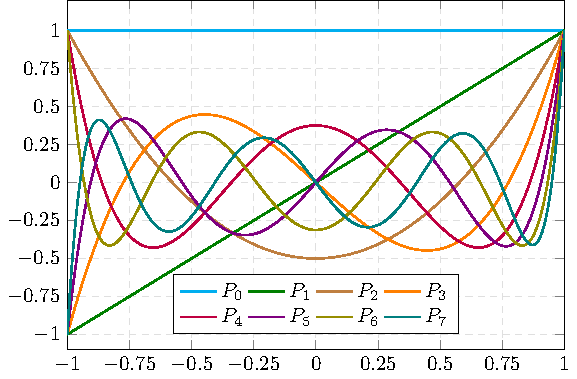
\includegraphics[width=\textwidth]{Images/legendre.pdf}
    \caption{Graphic representation of the first eight Legendre polynomials.}
  \end{minipage}
  \hfill
  \begin{minipage}[ht]{0.48\textwidth}
    \centering
    \captionsetup{type=table} %% tell latex to change to table
    \begin{tabular}{c|c}
      $n$ & $P_n(x)$                                 \\
      \hline\hline
      $0$ & $1$                                      \\
      $1$ & $x$                                      \\
      $2$ & $\frac{1}{2}(3x^2-1)$                    \\
      $3$ & $\frac{1}{2}(5x^3-3x)$                   \\
      $4$ & $\frac{1}{8}(35x^4-30x^2+3)$             \\
      $5$ & $\frac{1}{8}(63x^5-70x^3+15x)$           \\
      $6$ & $\frac{1}{16}(231x^6-315x^4+105x^2-5)$   \\
      $7$ & $\frac{1}{16}(429x^7-693x^5+315x^3-35x)$ \\
    \end{tabular}
    \caption{First eight Legendre polynomials}
    \label{tab:legendre_polys}
  \end{minipage}
\end{figure}
% The following proposition gives and explicit formula for the Legendre polynomials.
% \begin{proposition}[Rodrigues' formula]
%   Let $n\in \NN\cup\{0\}$. Then, $\forall x\in[-1,1]$:
%   \begin{equation}\label{eq:rodrigues}
%     P_n(x)=\frac{1}{2^n n!}\dv[n]{}{x}\left[{\left(x^2-1\right)}^n\right]
%   \end{equation}
% \end{proposition}
% \textcolor{red}{\begin{proposition}
%     Consider the function $g_x(t)=\frac{1}{\sqrt{1-2xt+t^2}}$ with $\abs{x}\leq 1$. Then, the generating function of $g$ is:
%     \begin{equation}
%       \frac{1}{\sqrt{1-2xt+t^2}}=\sum_{n=0}^{\infty}P_n(x)t^n
%     \end{equation}
%   \end{proposition}
%   \begin{proof}
%     Assume that formally $\frac{1}{\sqrt{1-2xt+t^2}}=\sum_{n=0}^{\infty}Q_n(x)t^n$. We want to check that $Q_n(x)=P_n(x)$ for all $n\in\NN\cup\{0\}$. Differentiating the equation with respect to $x$ and with respect to $t$ we obtain:
%     \begin{equation}\label{eq:rec_legendre_proof}
%       \frac{x-t}{{(1-2xt+t^2)}^{3/2}}=\sum_{n=0}^{\infty}nQ_n(x)t^{n-1}\qquad\frac{t}{{(1-2xt+t^2)}^{3/2}}=\sum_{n=0}^{\infty}{Q_n}'t^n
%     \end{equation}
%     The second equation can be rewritten as:
%     \begin{equation}
%       t\sum_{n=0}^{\infty}Q_n t^n=(1-2xt+t^2)\sum_{n=0}^{\infty}{Q_n}'(x)t^{n-1}
%     \end{equation}
%     So equating the coefficients of $t^n$ we get:
%     \begin{equation}
%       Q_{n}={Q_{n+1}}'-2x{Q_n}'+{Q_{n-1}}'
%     \end{equation}
%     Moreover, from \cref{eq:rec_legendre_proof} we have that:
%     \begin{equation}
%       t\sum_{n=0}^{\infty}nQ_n(x)t^{n-1}=(x-t)\sum_{n=0}^{\infty}{Q_n}'(x)t^{n}
%     \end{equation}
%     Again equating the coefficients of $t^n$ we get:
%     \begin{equation}
%       nQ_n=x{Q_n}'-{Q_{n-1}}'
%     \end{equation}
%     Hence differentiating $(1-x^2){P_n}'$ we have:
%     \begin{equation}
%       {((1-x^2){P_n}')}'=-2x{P_n}'+(1-x^2)P
%     \end{equation}
%     \textcolor{red}{NOT FINISHED!!!!!!!!!!}
%   \end{proof}}
The following proposition will be of our interest in the next section \cite{mathematical_methods}.
\begin{proposition}\label{prop:associate_legendre}
  Let $y(x)$ be a solution to the Legendre differential equation. Then, $\forall m\in\NN\cup\{0\}$ the function
  \begin{equation}
    w_m(x)={(1-x^2)}^{m/2} \dv[m]{y(x)}{x}
  \end{equation}
  solves the \emph{general Legendre differential equation}:
  \begin{equation}
    (1-x^2)y''-2xy'+\left(\lambda - \frac{m^2}{1-x^2}\right) y=0
  \end{equation}
  In particular if $\lambda=n(n+1)$ for $n\in\NN\cup\{0\}$, then $w_m(x)$ is denoted as
  \begin{equation}\label{eq:associated_legendre_polynomials}
    P_{n,m}(x):={(1-x^2)}^{m/2} \dv[m]{P_n}{x}
  \end{equation}
  and it is called the \emph{associated Legendre polynomial} of degree $n$ and order $m$.
\end{proposition}
% \begin{proof}
%   We know that $P_n$ satisfies the equation:
%   \begin{equation}\label{eq:proof_aso1}
%     (1-x^2)P_n''-2xP_n'+n(n+1)P_n=0
%   \end{equation}
%   Recall the Leibniz rule for differentiation:
%   \begin{equation}
%     {(fg)}^{(m)}=\sum_{k=0}^{m}\binom{m}{k}f^{(m-k)}g^{(k)}
%   \end{equation}
%   Differentiating \cref{eq:proof_aso1} $m$ times using the Leibniz rule and letting $v=\dv[m]{P_n}{x}$ we obtain:
%   \begin{equation}
%     [(1-x^2)v''-2xm v'-m(m-1)v]-[2xv'+2mv]+n(n+1)v= (1-x^2)v''-2x(m+1)v'+(n-m)(n+m+1)v=0
%   \end{equation}
%   Now let $P_{n,m}(x)={(1-x^2)}^{m/2}v$. Using the chain rule and isolating $v'$ and $v''$ we obtain:
%   \begin{align*}
%     {P_{n,m}}'= {(1-x^2)}^{m/2}v' - \frac{m}{2}x{(1-x^2)}^{m/2-1}v={(1-x^2)}^{m/2}v' - \frac{m}{2}\frac{P_{n,m}}{1-x^2}\implies v'= \frac{2}{m}\frac{1-x^2}{x}P_{n,m} - \frac{2}{m}x{P_{n,m}}' \\
%   \end{align*}
%   ....
% \end{proof}
Note that although we opted to call the functions $P_{n,m}$ as \emph{polynomials}, they are only \emph{true} polynomials when $m$ is even. But we have opted to call them in that manner as it is the common practice in the literature (see \cite{wolfram_associated_legendre_polynomials,mathematical_methods,florida:legendre}).

Moreover, from the definition of $P_{n,m}$, we can see $P_{n,0}=P_n$ and that $P_{n,m}=0$ if $m>n$. So we can restrict the domain of $m$ to the set $\{0,1,\dots,n\}$.

% Finally, putting \cref{eq:associated_legendre_polynomials,eq:rodrigues} together, we obtain the following explicit formula for the associated Legendre polynomials:
% \begin{equation}
%   P_{n,m}(x)=\frac{1}{2^n n!}{(1-x^2)}^{m/2} \dv[n+m]{x}\left[{\left(x^2-1\right)}^n\right]
% \end{equation}
% This allows us to extend the range of $m$ to $\{-n,-(n-1),\dots,n-1,n\}$.
% \begin{lemma}\label{lem:neg_asso_legendre}
%   Let $n\in\NN\cup\{0\}$ and $m\in\{0,\ldots,n\}$. Then:
%   \begin{equation}
%     P_n^{-m}(x)=(-1)^m \frac{(n-m)!}{(n+m)!}P_{n,m}(x)
%   \end{equation}
% \end{lemma}
% This lemma shows us that the new extended associated polynomials $P_n^{-m}$, $m\in\{0,\ldots,n\}$, are also solutions to the general Legendre differential equation because the satisfy the same equation as $P_{n,m}$ and they only differ by a constant factor.
% My spherical harmonics are the same as the ones in Riley, Hobson, Bence except for the minus sign (-1)^m in front of Y_{n,m}^{\mathrm{c}}.  
\begin{table}[ht]
  \centering
  \captionsetup{type=table} %% tell latex to change to table
  \begin{tabular}{c|c||c|c}
    $n$ & $P_{n,1}(x)$                              & $n$ & $P_{n,2}(x)$                          \\
    \hline
    $1$ & $\sqrt{1-x^2}$                            & $2$ & $3(1-x^2)$                            \\
    $2$ & $3x\sqrt{1-x^2}$                          & $3$ & $15x(1-x^2)$                          \\
    $3$ & $\frac{3}{2}(5 x^2-1)\sqrt{1-x^2}$        & $4$ & $\frac{15}{2}(7x^2-1)(1-x^2)$         \\
    $4$ & $\frac{5}{2}x(7x^2-3)\sqrt{1-x^2}$        & $5$ & $\frac{105}{2}x(3x^2-1)(1-x^2)$       \\
    $5$ & $\frac{15}{8}(21x^4-14x^2+1)\sqrt{1-x^2}$ & $6$ & $\frac{105}{8}(33x^4-18x^2+1)(1-x^2)$ \\
  \end{tabular}
  \caption{First associated Legendre polynomials for $m=1$ and $m=2$.}
\end{table}
\begin{figure}[ht]
  \centering
  \begin{subfigure}[b]{0.48\textwidth}
    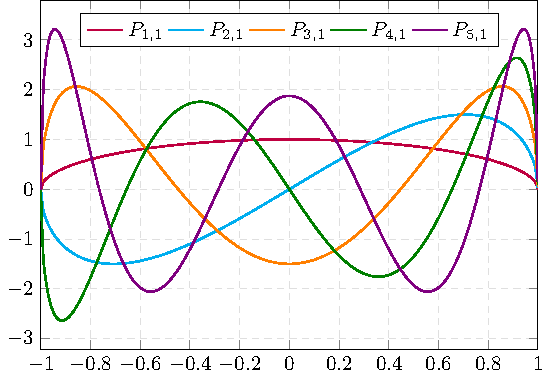
\includegraphics[width=\textwidth]{Images/assolegendre1.pdf}
    \caption{$m=1$}
  \end{subfigure}
  \quad
  \begin{subfigure}[b]{0.48\textwidth}
    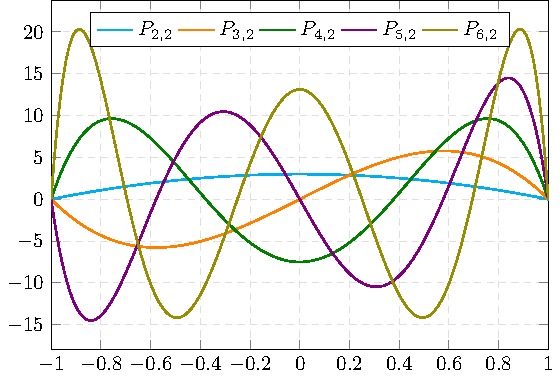
\includegraphics[width=\textwidth]{Images/assolegendre2.pdf}
    \caption{$m=2$}
  \end{subfigure}
  \caption{Graphic representation of the first associated Legendre polynomials for $m=1$ and $m=2$.}
\end{figure}
\begin{definition}
  Let $n\in\NN\cup\{0\}$ and $m\in\{0,1,\dots,n\}$. We define the \emph{real spherical harmonics} $Y_{n,m}^{\mathrm{c}}$ and $Y_{n,m}^{\mathrm{s}}$ as:
  \begin{align}
    Y_{n,m}^{\mathrm{c}}(\theta,\phi) & =\sqrt{(2-\delta_{0,m})(2n+1)\frac{(n-m)!}{(n+m)!} }P_{n,m}(\cos\phi) \cos{m\theta} \\
    Y_{n,m}^{\mathrm{s}}(\theta,\phi) & =\sqrt{(2-\delta_{0,m})(2n+1)\frac{(n-m)!}{(n+m)!} }P_{n,m}(\cos\phi) \sin{m\theta}
  \end{align}
  The factor $N_{n,m}:=\sqrt{(2-\delta_{0,m})(2n+1)\frac{(n-m)!}{(n+m)!} }$ is called the \emph{normalization factor} of the spherical harmonics and $\delta_{0,m}$ is the Kronecker delta. The weird factor $2-\delta_{0,m}$ in $N_{n,m}$ will become clear in the next section.
\end{definition}
\begin{table}[ht]
  \centering
  \captionsetup{type=table} %% tell latex to change to table
  \begin{tabular}{c|c|c||c|c|c}
    $n$ & $m$ & $Y_{n,m}^{\mathrm{c}}(\theta,\phi)$     & $n$ & $m$ & $Y_{n,m}^{\mathrm{c}}(\theta,\phi)$                        \\
    \hline
    $0$ & 0   & $1$                                     & $2$ & 2   & $\frac{\sqrt{15}}{2}{(\sin\phi)}^2\cos 2\theta$            \\
    $1$ & 0   & $\sqrt{3}\cos\phi$                      & $3$ & 0   & $\frac{\sqrt{7}}{2}\cos\phi(5{(\cos\phi)}^2-3)$            \\
    $1$ & 1   & $\sqrt{3}\sin\phi\cos\theta$            & $3$ & 1   & $\frac{\sqrt{42}}{4}(5{(\cos\phi)}^2-1)\sin\phi\cos\theta$ \\
    $2$ & 0   & $\frac{\sqrt{5}}{2}(3{(\cos\phi)}^2-1)$ & $3$ & 2   & $\frac{\sqrt{105}}{2}{(\sin\phi)}^2\cos\phi\cos 2\theta$   \\
    $2$ & 1   & $\sqrt{15}\sin\phi\cos\phi\cos\theta$   & $3$ & 3   & $\frac{\sqrt{70}}{4}{(\sin\phi)}^3\cos 3\theta$            \\
  \end{tabular}
  \caption{First cosine spherical harmonics.}
\end{table}
\begin{figure}[ht]
  \centering
  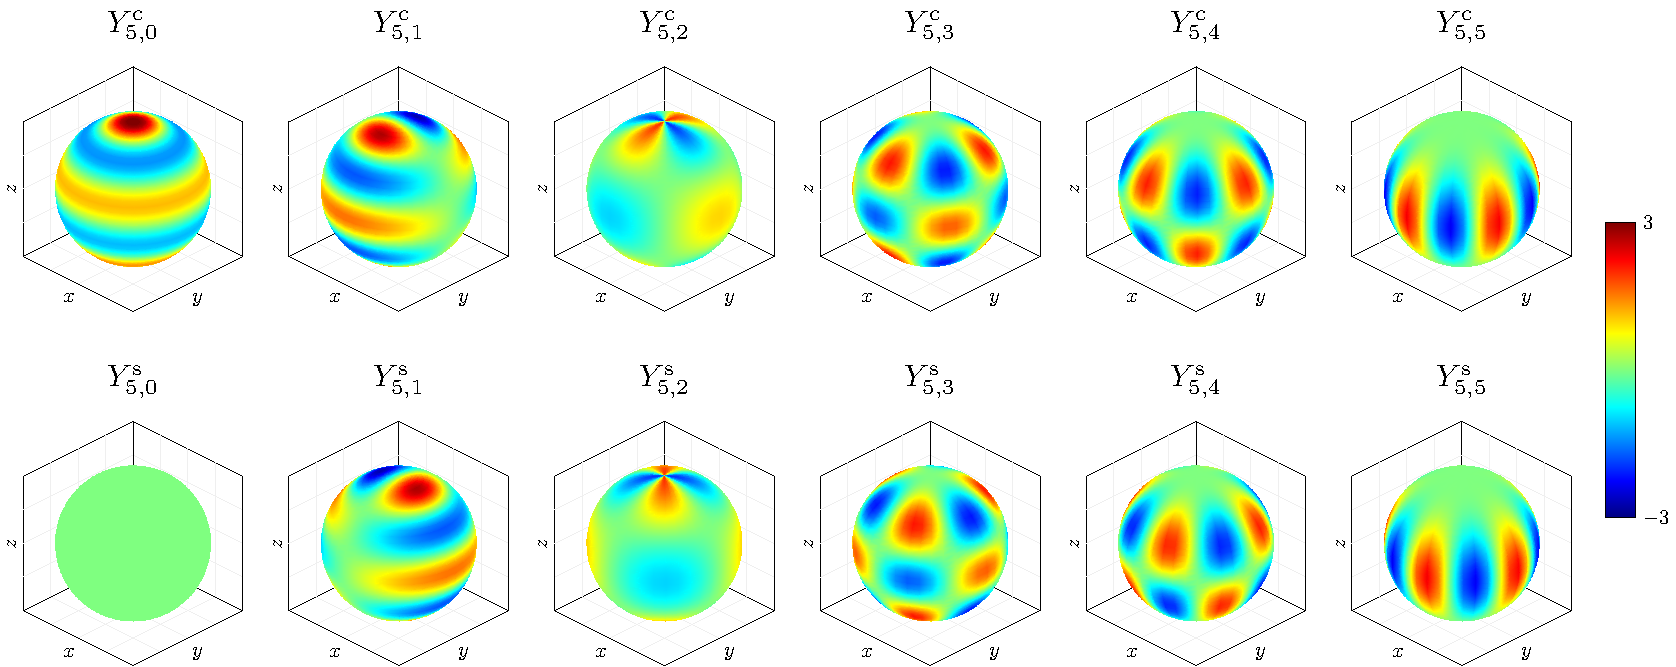
\includegraphics[width=\textwidth]{Images/sphericalHarmonics.pdf}
  \caption{3D heat map of the spherical harmonics of degree $n=5$. The first row correspond to the cosine spherical harmonics and the second row correspond to the sine spherical harmonics.}
\end{figure}

\subsubsection{Laplace's equation in spherical coordinates}\label{sec:laplace_spherical}
\begin{definition}
  Let $f:\RR^3\rightarrow\RR$ be a twice-differentiable function. The \emph{Laplace equation} is the equation
  \begin{equation}
    \laplacian f=\pdv[2]{f}{x}+\pdv[2]{f}{y}+\pdv[2]{f}{z}=0
  \end{equation}
  where $\Delta$ is the Laplace operator.
\end{definition}
The next proposition gives the Laplace equation in spherical coordinates.
\begin{proposition}
  Let $f:\RR^3\rightarrow\RR$ be a twice-differentiable function. Then:
  \begin{equation}\label{eq:laplace}
    \frac{1}{r^2}\pdv{}{r}\left(r^2\pdv{f}{r}\right)+\frac{1}{r^2\sin\phi}\pdv{}{\phi}\left(\sin\phi\pdv{f}{\phi}\right)+\frac{1}{r^2{(\sin\phi)}^2}\pdv[2]{f}{\theta}=0
  \end{equation}
  where $r\in[0,\infty)$ denotes the radial distance, $\theta\in[-\pi,\pi)$ denotes the longitude, and $\phi\in[0,\pi]$, the colatitude:
  \begin{equation}
    \begin{aligned}
      x & =r\sin\phi\cos\theta \\
      y & =r\sin\phi\sin\theta \\
      z & =r\cos\phi
    \end{aligned}
  \end{equation}
\end{proposition}
We are now interested in solving the Laplace equation. \cref{thm:laplace_spherical} gives the solution of it as a function of the spherical harmonics.
\begin{theorem}\label{thm:laplace_spherical}
  The regular solutions in a bounded region $\Omega\subseteq \RR^3$ such that $0\notin\overline{\Omega}$ of the Laplace equation in spherical coordinates are of the form
  \begin{align}
    f(r,\theta,\phi) & = \sum_{n=0}^\infty \sum_{m=0}^n (a_n r^{n} +b_{n}r^{-n-1})P_{n,m}(\cos\phi) (c_{n,m}\cos(m\theta)+s_{n,m}\sin(m\theta))                                                              \\
                     & \label{eq:sol_laplace} = \sum_{n=0}^\infty \sum_{m=0}^n (a_n r^{n} +b_{n}r^{-n-1})(\tilde{c}_{n,m}Y_{n,m}^{\mathrm{c}}(\theta,\phi)+\tilde{s}_{n,m}Y_{n,m}^{\mathrm{s}}(\theta,\phi))
  \end{align}
  where $a_n,b_n,c_{n,m},s_{n,m},\tilde{c}_{n,m},\tilde{s}_{n,m}\in\RR$.
\end{theorem}
\begin{proof}
  Let $f(r,\theta,\phi)$ be a solution of \cref{eq:laplace} Using separation variables $f(r,\theta,\phi)=R(r)\Theta(\theta)\Phi(\phi)$ we can write:
  \begin{equation}
    \frac{\Theta\Phi}{r^2}{(r^2R')}'+\frac{R\Theta}{r^2\sin\phi}{(\sin\phi\Phi')}'+\frac{R\Phi}{r^2{(\sin\phi)}^2}\Theta''=0
  \end{equation}
  Here we are making and abuse of notation denoting all the derivative with a prime, but the reader should have no confusion with it. Isolating $R$ from $\Theta$ and $\Phi$ yields:
  \begin{equation}
    \frac{{(r^2R')}'}{R}=-\frac{1}{\sin\phi\Phi}{(\sin\phi\Phi')}'-\frac{1}{{(\sin\phi)}^2\Theta}\Theta''
  \end{equation}
  Since the left-hand side depends entirely on $r$ and the right-hand side does not, it follows that both sides must be constant. Therefore:
  \begin{align}
    \label{eq:laplaceR}        & \frac{{(r^2R')}'}{R}=\lambda                                                               \\
    \label{eq:laplaceThetaPhi} & \frac{1}{\sin\phi\Phi}{(\sin\phi\Phi')}'+\frac{1}{{(\sin\phi)}^2\Theta}\Theta''  =-\lambda
  \end{align}
  with $\lambda\in\RR$. Similarly, separating variables from \cref{eq:laplaceThetaPhi} we obtain that the equations
  \begin{align}
    \label{eq:laplaceTheta} & \frac{1}{\Theta}\Theta''  =-m^2                                     \\
    \label{eq:laplacePhi}   & \frac{\sin\phi}{\Phi}{(\sin\phi\Phi')}'+\lambda{(\sin\phi)}^2  =m^2
  \end{align}
  must be constant with $m\in\CC$ (a priori). The solution to the well-known \cref{eq:laplaceTheta} is a linear combination of the $\cos(m\theta)$ and $\sin(m\theta)$. Note, though, that since $\Theta$ must be a $2\pi$-periodic function, that is satisfying $\Theta(\theta+2\pi)=\Theta(\theta)$ $\forall\theta\in\RR$, $m$ must be an integer. On the other hand making the change of variables $x=\cos \phi$ and $y=\Phi(\phi)$ in \cref{eq:laplacePhi} and using the chain rule, that equation becomes:
  \begin{equation}\label{}
    (1-x^2)\dv[2]{y}{x}-2x\dv[2]{y}{x}+\left(\lambda-\frac{m^2}{1-x^2}\right)y=0
  \end{equation}
  which is the associate Legendre equation. We have argued in \cref{prop:associate_legendre} that we need $\lambda=n(n+1)$ and $m\leq n$ in order to get regular solutions at $x=\cos\phi=\pm 1$. Moreover, these solutions are $P_{n,m}(\cos\phi)$.

  Finally, note that equation \cref{eq:laplaceR} is a Cauchy-Euler equation (check \cite{wiki:cauchy-euler}) and so the general solution of it is given by
  \begin{equation}
    R(r) = c_1 r^{n} + c_2 r^{-n-1}
  \end{equation}
  because $\lambda = n(n+1)$ (the reader may check that $r^n$ and $r^{-n-1}$ are indeed two independent solutions of \cref{eq:laplaceR}). So the general solution becomes a linear combination of each solution founded varying $n\in\NN\cup\{0\}$ and $m\in\{0,1,\dots,n\}$:
  \begin{equation}
    f(r,\theta,\phi) = \sum_{n=0}^\infty \sum_{m=0}^n (a_n r^{n} +b_{n}r^{-n-1})P_{n,m}(\cos\phi) (c_{n,m}\cos(m\theta)+s_{n,m}\sin(m\theta))
  \end{equation}
\end{proof}
From now we are not concerning on the singularity at $r=0$ of \cref{eq:sol_laplace} (see \cref{sec:laplace_spherical_potential} for more details).

The associated Legendre polynomials satisfy an orthogonality relation:
\begin{lemma}\label{lem:ortho_asso_legendre}
  Let $n_1,n_2\in\NN\cup\{0\}$ and $m\leq \min\{n_1,n_2\}$. Then:
  \begin{equation}
    \int_0^1 P_{n_1,m}(x) P_{n_2,m}(x) \dd{x}=\frac{2}{2n_1+1}\frac{(n_1+m)!}{(n_1-m)!} \delta_{n_1,n_2}
  \end{equation}
  where $\delta_{n_1,n_2}$ denotes the Kronecker delta.
\end{lemma}
Similarly, it can be shown that the spherical harmonics from an orthonormal family of functions:
\begin{proposition}
  The family of spherical harmonics $\{Y_{n,m}^{\mathrm{c}}(\theta,\phi),Y_{n,m}^{\mathrm{s}}(\theta,\phi):n\in\NN\cup\{0\},m\leq n\}$ is orthonormal in the following sense:
  \begin{equation}\label{eq:ortho_spherical_harmonics}
    \frac{1}{4\pi}\int_0^{2\pi}\int_0^\pi Y_{n_1,m_1}^i(\theta,\phi) Y_{n_2,m_2}^j(\theta,\phi)\dd\Omega=\delta_{n_1,n_2}\delta_{m_1,m_2}\delta_{i,j}
  \end{equation}
  where $\dd\Omega=\sin\phi\dd{\phi}\dd{\theta}$ is the solid angle element, which measures the element of area on a sphere of radius $1$.
\end{proposition}
\begin{proof}
  Let $N_{n_1,m_1}$, $N_{n_2,m_2}$ be the normalization factors of the spherical harmonics $Y_{n_1,m_1}$, $Y_{n_2,m_2}$ respectively. Note that we can separate the variables in the integral of \cref{eq:ortho_spherical_harmonics}. So if $i\ne j$, the integral over $\theta$ becomes $\int_0^{2\pi}\cos(m_1\theta)\sin(m_2\theta)\dd{\theta}$ which is equal to 0 regardless of the values of $m_1$ and $m_2$. So from now on assume that $i=j$. Due to the symmetry between the cosine and the sine we can suppose that $i=\mathrm{c}$. Thus:
  \begin{multline}
    \int_0^{2\pi}\int_0^\pi Y_{n_1,m_1}^i(\theta,\phi) Y_{n_2,m_2}^j(\theta,\phi)\dd\Omega=\\= N_{n_1,m_1}N_{n_2,m_2}\int_0^\pi P_{n_1,m_1}(\cos\phi) P_{n_2,m_2}(\cos\phi)\sin\phi\dd\phi\int_{0}^{2\pi}\cos(m_1\theta)\cos(m_2\theta)\dd{\theta}
  \end{multline}
  An easy check shows that if $m_1\neq m_2$ then the integral over $\theta$ is zero (and the same applies with sines). So suppose $m_1=m_2=m$. In that case, if $m\ne 0$ we have $\int_{0}^{2\pi}{(\cos m\theta)}^2\dd{\theta}=\int_{0}^{2\pi}{(\sin m\theta)}^2\dd{\theta}=\pi$ and if $m=0$, the cosine integral evaluates to $2\pi$ whereas the sine integral is 0. We can omit this latter case because $Y_{n,0}^{\mathrm{s}}$ is identically zero. Thus:
  \begin{equation}
    \frac{2\pi}{2-\delta_{0,m}} N_{n_1,m}N_{n_2,m}\int_0^\pi P_{n_1,m}(\cos\phi) P_{n_2,m}(\cos\phi)\sin\phi\dd\phi=\frac{2\pi}{2-\delta_{0,m}} N_{n_1,m}N_{n_2,m}\int_{-1}^1 P_{n_1,m}(x) P_{n_2,m}(x)\dd{x}
  \end{equation}
  By \cref{lem:ortho_asso_legendre} this latter integral is $\frac{2}{2n_1+1}\frac{(n_1+m)!}{(n_1-m)!} \delta_{n_1,n_2}$. Finally, if $n_1=n_2=n$, putting all normalization factors together we get:
  \begin{equation}
    \frac{2\pi}{2-\delta_{0,m}} N_{n}^{m}N_{n}^{m}\frac{2}{2n+1}\frac{(n+m)!}{(n-m)!}=4\pi
  \end{equation}
\end{proof}
Moreover, an important result in the Sturm-Liouville Theory of second order differential equations (\cite{wiki:sturmliouville,completenessSL}) says that the family of spherical harmonics $\{Y_{n,m}^{\mathrm{c}}(\theta,\phi),Y_{n,m}^{\mathrm{s}}(\theta,\phi):n\in\NN\cup\{0\},m\leq n\}$ form a complete set in the sense that any smooth function defined on the sphere $f:S^2\rightarrow\RR$ can be expanded in a series of spherical harmonics:
\begin{equation}
  f(\theta,\phi)=\sum_{n=0}^\infty\sum_{m=0}^n (c_{n,m} Y_{n,m}^{\mathrm{c}}(\theta,\phi)+s_{n,m} Y_{n,m}^{\mathrm{s}}(\theta,\phi))
\end{equation}
This will be useful in \cref{sec:laplace_spherical_potential} when expanding the gravitational potential created by the Earth at some arbitrary point in spherical harmonics.

\subsubsection{Expansion in spherical harmonics}\label{sec:laplace_spherical_potential}
We have just seen that $V$ satisfies the exterior Dirichlet problem for the Laplace equation. In \cref{sec:laplace_spherical} we saw that a solution to the Laplace equation can be expressed as:
\begin{equation}\label{eq:prePotential}
  V(r,\theta,\phi) = \sum_{n=0}^\infty \sum_{m=0}^n (a_n r^{n} +b_{n}r^{-n-1})(\tilde{c}_{n,m}Y_{n,m}^{\mathrm{c}}(\theta,\phi)+\tilde{s}_{n,m}Y_{n,m}^{\mathrm{s}}(\theta,\phi))
\end{equation}
where $a_n,b_n,\tilde{c}_{n,m},\tilde{s}_{n,m}\in\RR$. If we impose $V$ to satisfy the third condition of \cref{eq:dirichletProblem}, we must have $a_{n}=0$.
Finally, if we choose $R_\oplus$ as a reference radius for a spherical model of the Earth, using the boundary condition on $\Fr{\Omega}$
\begin{equation}
  f(\theta,\phi) = \sum_{n=0}^\infty \sum_{m=-n}^n \frac{b_{n}}{{R_\oplus}^{n+1}}(\tilde{c}_{n,m}Y_{n,m}^{\mathrm{c}}(\theta,\phi)+\tilde{s}_{n,m}Y_{n,m}^{\mathrm{s}}(\theta,\phi))
\end{equation}
and the orthogonality of the spherical harmonics, we can deduce that the coefficients $b_n\tilde{c}_{n,m}$ and $b_n\tilde{s}_{n,m}$ are given by:
\begin{align}
  b_n\tilde{c}_{n,m} & =\frac{{R_\oplus}^{n+1}}{4\pi}\int_0^{2\pi}\int_0^\pi f(\theta,\phi) Y_{n,m}^\mathrm{c}(\theta,\phi)\sin\phi\dd{\phi}\dd{\theta} \\
  b_n\tilde{s}_{n,m} & =\frac{{R_\oplus}^{n+1}}{4\pi}\int_0^{2\pi}\int_0^\pi f(\theta,\phi) Y_{n,m}^\mathrm{s}(\theta,\phi)\sin\phi\dd{\phi}\dd{\theta}
\end{align}

Hence, introducing the gravitational constant $G$ and the Earth's mass $M_\oplus$ into the equation, our final expression for the gravitational potential is
\begin{equation}\label{eq:Potential}
  V(r,\theta,\phi) =\frac{GM_\oplus}{R_\oplus}\sum_{n=0}^\infty \sum_{m=0}^n{\left(\frac{{R_\oplus}}{r}\right)}^{n+1}(\bar{C}_{n,m}Y_{n,m}^{\mathrm{c}}(\theta,\phi)+\bar{S}_{n,m}Y_{n,m}^{\mathrm{s}}(\theta,\phi))
\end{equation}
where the coefficients $\bar{C}_{n,m},\bar{S}_{n,m}\in\RR$ are given by the formulas:
\begin{align}
  \bar{C}_{n,m} & =\frac{1}{4\pi}\frac{R_\oplus}{G M_\oplus}\int_0^{2\pi}\int_0^\pi f(\theta,\phi)  Y_{n,m}^\mathrm{c}(\theta,\phi)\sin\phi\dd{\phi}\dd{\theta} \\
  \bar{S}_{n,m} & =\frac{1}{4\pi}\frac{R_\oplus}{G M_\oplus}\int_0^{2\pi}\int_0^\pi f(\theta,\phi)  Y_{n,m}^\mathrm{s}(\theta,\phi)\sin\phi\dd{\phi}\dd{\theta}
\end{align}
% My coefficients Cnm and Snm are the \bar{Cnm} and \bar{Snm} in Montebruck book

The coefficients $\bar{C}_{n,m}$, $\bar{S}_{n,m}$ are called \emph{geopotential coefficients}, and they describe the dependence on the Earth's internal structure. They are obtained from observation of the perturbations seen in the orbits of other satellites \cite{montenbruck}. Other methods for obtaining such data are through surface gravimetry, which provides precise local and regional information about the gravity field, or through altimeter data, which can be used to provide a model for the geoid of the Earth, that is the shape that the ocean surface would take under the influence of the gravity of Earth, which in turn can be used to obtain the geopotential coefficients.
\subsection{Numerical computation of the gravity acceleration}
Up to this point, we have only studied the gravitational potential exerted by the non-homogeneous Earth on a satellite. But, in order to integrate the equations of motion of the satellite, we need to compute the gravitational acceleration $\vf{g}=-\grad{V}$ instead. In order to do this efficiently, we will make use of the following formulas given in \cite{montenbruck,cunningham}. First, let
\begin{equation}
  V_{n,m}(\theta,\phi)={\left(\frac{R_\oplus}{r}\right)}^{n+1} P_{n,m}(\cos\phi)\cos(m \theta)\qquad W_{n,m}(\theta,\phi)={\left(\frac{R_\oplus}{r}\right)}^{n+1} P_{n,m}(\cos\phi)\sin(m \theta)
\end{equation}
Thus, we can write:
\begin{equation}
  V=\sum_{n=0}^\infty \sum_{m=0}^n \bar{C}_{n,m}N_{n,m} V_{n,m}+\bar{S}_{n,m}N_{n,m} W_{n,m}
\end{equation}
Let $C_{n,m}:= \bar{C}_{n,m}N_{n,m}$ and $ S_{n,m}:= \bar{S}_{n,m}N_{n,m}$. If $\vf{g}=(\ddot{x}, \ddot{y}, \ddot{z})$, then:
\begin{equation}
  \ddot{x} = \sum_{n=0}^\infty \sum_{m=0}^n\ddot{x}_{n,m}\qquad \ddot{y} = \sum_{n=0}^\infty \sum_{m=0}^n\ddot{y}_{n,m}\qquad \ddot{z} = \sum_{n=0}^\infty \sum_{m=0}^n\ddot{z}_{n,m}
\end{equation}
where the \textit{partial} accelerations $x_{n,m}$, $y_{n,m}$, $z_{n,m}$ are given by:
\begin{align}
  \ddot{x}_{n,m} & =\begin{cases}
                      \displaystyle-\frac{GM_\oplus}{{R_\oplus}^2}C_{n,0}V_{n+1,1}                                                                                         & \text{ if $m=0$} \\[10pt]
                      \begin{aligned}[b]
      \displaystyle-\frac{GM_\oplus}{{R_\oplus}^2}\bigg[C_{n,m}V_{n+1,m+1}+ S_{n,m}W_{n+1,m+1}-\hspace{4cm} \\
      -  \frac{{(n-m+2)}!}{{(n-m)}!}\left(C_{n,m}V_{n+1,m-1}+S_{n,m}W_{n+1,m-1}\right)\bigg]
    \end{aligned} & \text{ if $m>0$}
                    \end{cases} \\
  \ddot{y}_{n,m} & =\begin{cases}
                      \displaystyle-\frac{GM_\oplus}{{R_\oplus}^2}C_{n,0}W_{n+1,1}                                                                                       & \text{ if $m=0$} \\[10pt]
                      \begin{aligned}
      \displaystyle -\frac{GM_\oplus}{{R_\oplus}^2}\bigg[C_{n,m}W_{n+1,m+1}-S_{n,m}V_{n+1,m+1}-\hspace{4cm} \\
      -\frac{{(n-m+2)}!}{{(n-m)}!}\left(C_{n,m}W_{n+1,m-1}-S_{n,m}V_{n+1,m-1}\right)\bigg]
    \end{aligned} & \text{ if $m>0$}
                    \end{cases}   \\
  \ddot{z}_{n,m} & =-\frac{GM_\oplus}{{R_\oplus}^2}(n-m+1)\left(C_{n,m}V_{n+1,m}+S_{n,m}W_{n+1,m}\right)
\end{align}
and the functions $V_{n,m}$, $W_{n,m}$ are calculated using the following recurrence relations:
\begin{align*}
  \begin{cases}
    \hspace{8pt}\begin{aligned}
                  V_{n,m} & =\frac{2n-1}{n-m} \frac{R_\oplus}{r}\cos\phi V_{n-1,m}-\frac{n+m-1}{n-m}\frac{{R_\oplus}^2}{r^2}V_{n-2,m} \\[0.1cm]
                  W_{n,m} & =\frac{2n-1}{n-m} \frac{R_\oplus}{r}\cos\phi W_{n-1,m}-\frac{n+m-1}{n-m}\frac{{R_\oplus}^2}{r^2}W_{n-2,m}
                \end{aligned} & \text{if $0\leq m\leq n-2$} \\[0.9cm]
    \begin{aligned}
      V_{n,n-1} & =(2n-1) \frac{R_\oplus}{r}\cos\phi V_{n-1,n-1} \\[0.1cm]
      W_{n,n-1} & =(2n-1) \frac{R_\oplus}{r}\cos\phi W_{n-1,n-1}
    \end{aligned}                                                                                       & \text{if $m=n-1$}                                               \\[0.9cm]
    \hspace{10.25pt}\begin{aligned}
                      V_{n,n} & =(2m-1)\frac{R_\oplus}{r}\sin\phi[\cos\theta V_{n-1,n-1}-\sin\theta W_{n-1,n-1}] \\[0.1cm]
                      W_{n,n} & =(2m-1)\frac{R_\oplus}{r}\sin\phi[\cos\theta W_{n-1,n-1}+\sin\theta V_{n-1,n-1}]
                    \end{aligned}                 & \text{if $m=n$}
  \end{cases}
\end{align*}
starting from the initial quantities $V_{00}= \frac{R_\oplus}{r}$ and $W_{00}= 0$.
\subsection{Other perturbations}
atmospheric drag, solar radiation pressure, and the gravitational pull of the Moon and Sun,
POSAR-HO SI AL FINAL FAIG SIMULACIO AMB AIXO, SI NO, NOOOO.

% From  https://physics.stackexchange.com/questions/19477/earth-centered-inertial-eci-reference-frame-as-approximate-inertial-frame-of-r
ECI coordinate frames are not truly inertial since the Earth itself is accelerating as it travels in its orbit about the Sun. In many cases, it may be assumed that the ECI frame is inertial without adverse effect. However, when computing the gravitational influence of a third body such as the Moon on the dynamics of a spacecraft, the acceleration of the ECI frame must be considered. For example, when computing the acceleration of an Earth-orbiting spacecraft due to the gravitational influence of the Moon, the acceleration of the Earth itself due to the Moon's gravity must be subtracted
\end{document}